\subsection{Creating and Using the \acrshort{ast}}\label{CreatingAst}

The goal for the \acrshort{ast} is to decrease the information in the tree.
The hidden information is then contained in fields created for the respective classes.
Rather than having the information as fields one could also choose to have this information as children of the nodes.
This would mean that to find the information one would have to run through the children of the node whereas the method chosen for this compiler, this information is kept on the fields of a node.
The advantage being that the information is kept together without clustering the tree.
All the nodes of the \acrshort{ast} have been designed with this in mind.
For example on figure \myref{image:ASTDecl} a class structure can be seen, which consists of all the classes needed to express a declaration on the tree.
A declaration could be \texttt{int a = 5;}.

\begin{figure}[!ht]
\centering
 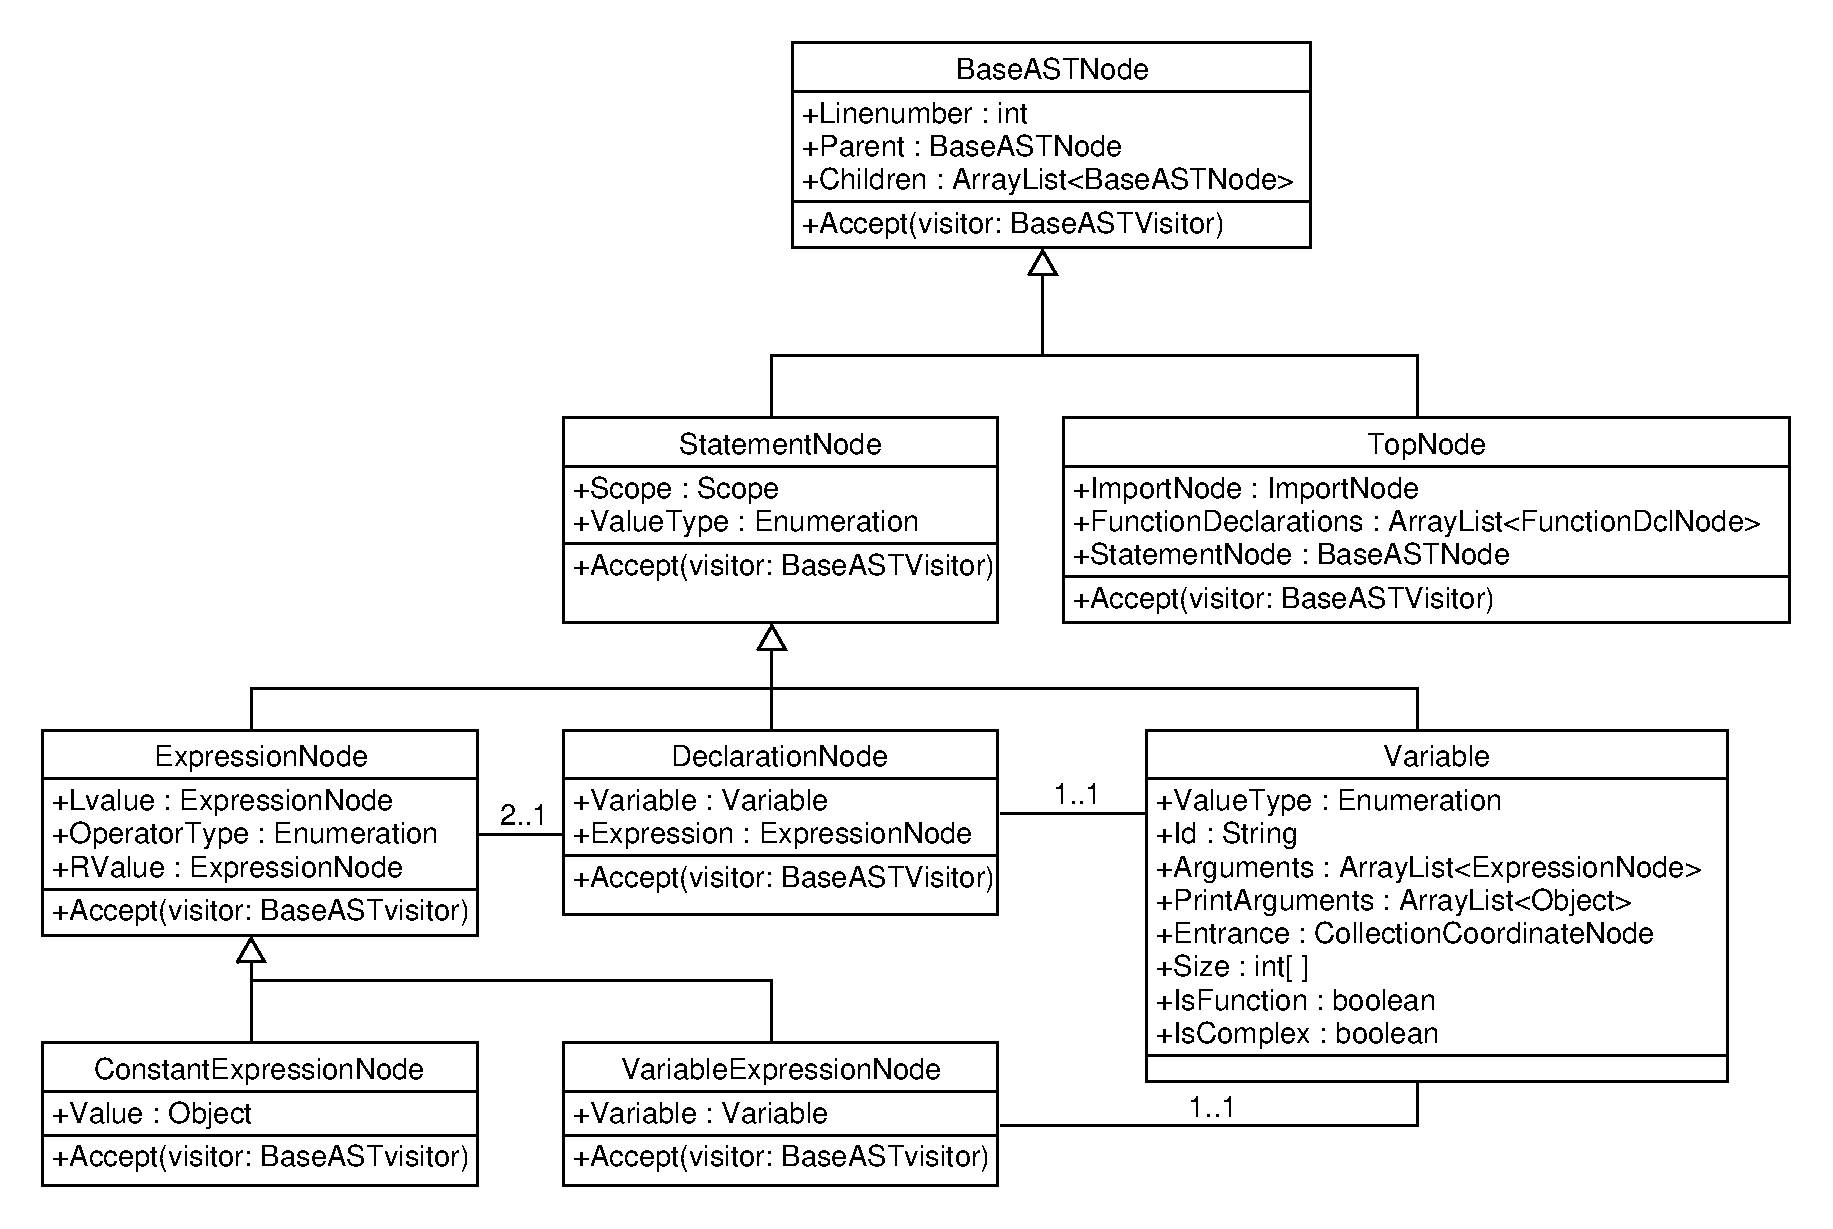
\includegraphics[width=1\textwidth]{figures/ClassDiagrams/ASTDeclarationNodeMoreInfo.pdf} % trim=4.85cm 15cm 0.85cm 1cm
\caption{A UML class diagram of the classes used for a DeclarationNode on the \acrshort{ast}.}\label{image:ASTDecl}
\vspace{-15pt}
\end{figure}

The \texttt{Variable} class contains a lot of different information which is used depending on which class a given instance of \texttt{Variable} is connected to.
If \texttt{Variable} is connected to a VariableExpressionNode, the only fields used on the variable class is ValueType and Id, while the booleans IsFunction and IsComplex are set to false.
In the example \texttt{int a = 5;} the tree structure looks like the AST on \myref{image:AST}.
When the right hand side of an assignment or declaration is a function, an example being \texttt{int a = foo(5);} the fields used on \texttt{Variable} differs from the previous example and instead becomes Id, ValueType, arguments, and the boolean IsFunction is instead set to true.
The printargument field is used when a functioncall to \texttt{Print();}is made. 
Entrance, Size and IsComplex are used when dealing with the complex data types, vectors and matrices.
\texttt{TopNode} sets the structure of a \gls{gamble} program as described in \myref{subsec:Struc}.
The full Classdiagram can be seen in \myref{ASTNodes}.

The classes have made it more intuitive to perform a traversal of the tree based upon the names of the fields on the classes.
E.g. the \texttt{ForLoopNode} has fields named \texttt{Body}, \texttt{Initialize}, \texttt{Update}, and \texttt{Conditional}, these names have meaning instead of just being children on the node which will be helpfull when implementing the rest of the compiler.

The Class \texttt{VisitorAST} creates the \acrshort{ast} from the parse tree, it traverses the tree using the visitor pattern and on every node sets a field of a class in the \acrshort{ast}. 
Afterwards the node is placed on the tree as a leaf or a field on the node which made the visit call.

One of these visit methods can be seen on \myref{lst:VisitorASTCode}.

\begin{lstlisting}[caption=The Visit Method for WhileLoopNode,frame=tlrb,label={lst:VisitorASTCode}]
public BaseASTNode visitWhileLoop(ourLangParser.WhileLoopContext ctx) {
    WhileLoopNode whileLoopNode = new WhileLoopNode(parentStack.peek());
    whileLoopNode.setCondNode(
    	(ConditionalExpressionNode)visit(ctx.conditionalExpression()));
    parentStack.push(whileLoopNode);
    visitChildren(ctx.whileBlock);
    parentStack.pop();
    whileLoopNode.setLineNumber(ctx.start.getLine());
    return whileLoopNode;
}
\end{lstlisting}
A stack called the parentstack is used to keep track of the caller to \texttt{visit()}, in order to keep track of the parents and the children of the tree.
On lines three and four a call to visit the conditionalexpression of the whileloop is made, which returns an instance of the class \texttt{ConditionalExpressionNode}.
Afterwards, to set the body of the \texttt{WhileLoopNode}, all the children of the nodes are visited, but first the \texttt{WhileLoopNode} is pushed to the parentstack.
This makes it possible to check which node is the parent of the children being created during the calls to visit.

While implementing the Visitor pattern for the \acrshort{ast} an interface was made, which contains a visit method for every single class of the \acrshort{ast}.
A baseclass was then been made which implements this interface.
The baseclass implements each visit method such that the correct fields of the nodes are visited in the correct order.
This means that any visitor class only has to override the visit methods which are of interest for the specific visitor.
An UML diagram for the implementations of the visitor pattern in the compiler and can be seen on \myref{image:Visitors}.
The figure shows how every visitor class inherits from the \texttt{BaseASTVisitor} class.

\begin{figure}[!ht]
\centering
 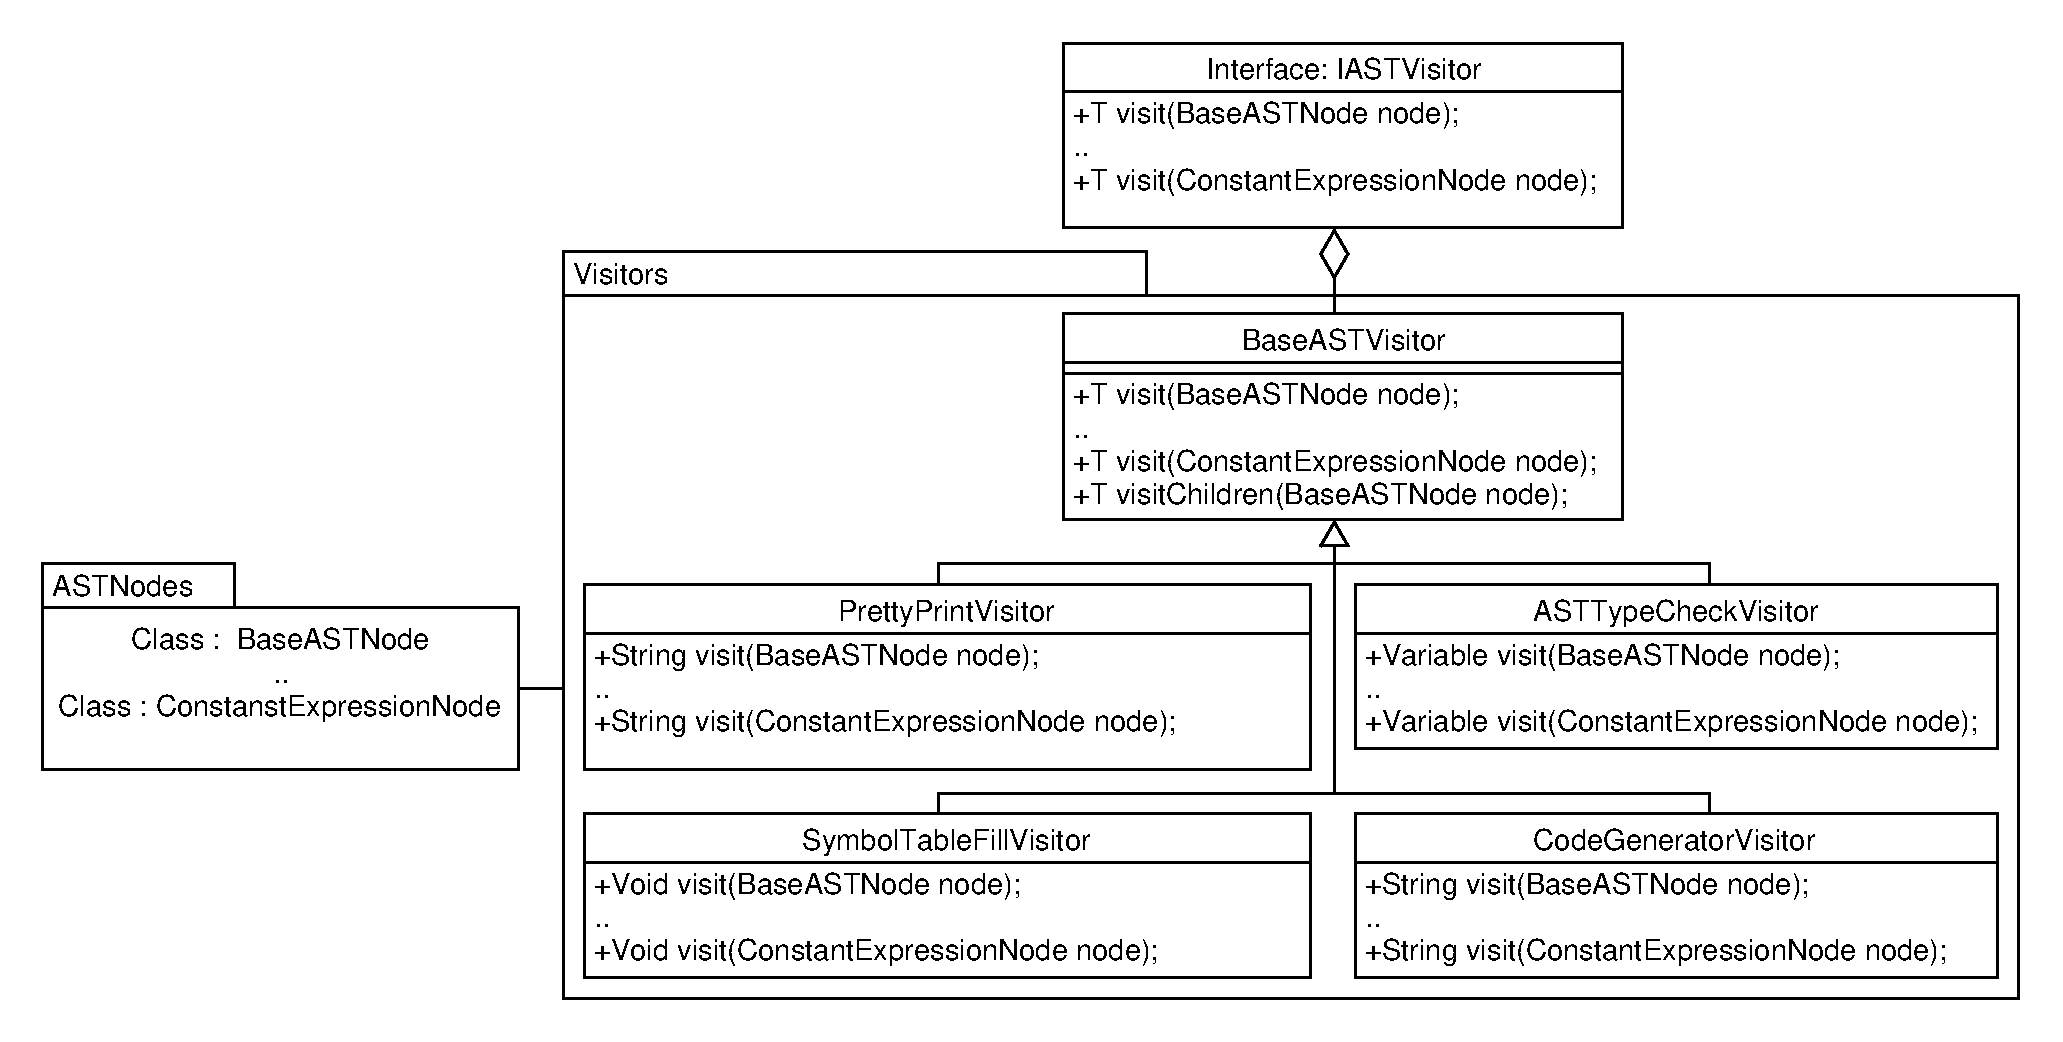
\includegraphics[width=1\textwidth]{figures/ClassDiagrams/Visitors.pdf} % trim=4.85cm 15cm 0.85cm 1cm
\caption{A UML diagram of the visitor patterns implementation in the compiler for traversing the \acrshort{ast}.}\label{image:Visitors}
\vspace{-15pt}
\end{figure} 